\documentclass{article}

\usepackage{amsmath,amssymb,amsthm,graphicx,subfigure}

\pagestyle{myheadings}

\pdfpagewidth 8.5in
\pdfpageheight 11 in

\setlength\topmargin{0in}
\setlength\textheight{8.5in}
\setlength\textwidth{6.5in}
\setlength\oddsidemargin{0in}
\setlength\evensidemargin{0in}

\newcommand{\suchthat}{\ni}
\newcommand{\onlyif}{\Longleftrighttriangle}
\newcommand{\definedby}{\triangleq}
\newcommand{\union}{\bigcup}
\newcommand{\intersect}{\bigcap}
\newcommand{\where}{\mid}
\newcommand{\inverse}{\overline}

\title{CIT 596 Homework 2}
\author{Steven Tomcavage\\stomcava@seas.upenn.edu}
\date{February 9, 2011}

\markboth{\hfill Steven Tomcavage }{\hfill Steven Tomcavage }

\begin{document}

\maketitle

\section{}

Give the state tables ($\delta$) for the FSMs given (omitted). 

Note: I've included the output for each transition following the name of the
state being transitioned to.

\subsection{}

State machine described by $\{Q, \Sigma, \delta, q_0, F\}$ where $Q = \{S_0,
S_1, S_2\}, \Sigma = \{0, 1\}, q_0 = S_0, F = \{\}, \text{ and } \delta
\text{ is:}$

\begin{table}[h!]
	\centering
	\begin{tabular}{ l || c | c }
	      & 0        & 1 \\
	\hline      
	$S_0$ & $S_1$, 0 & $S_2$, 1  \\
	$S_1$ & $S_2$, 0 & $S_1$, 0  \\
	$S_2$ & $S_2$, 1 & $S_0$, 0  \\
	\end{tabular}
	\caption{State transition table for FSM given in problem 1a.}
	\label{table_1a}
\end{table}

\subsection{}

State machine described by $\{Q, \Sigma, \delta, q_0, F\}$ where $Q = \{S_0,
S_1, S_2, S3\}, \Sigma = \{0, 1\}, q_0 = S_0, F = \{\}, \text{ and } \delta
\text{ is:}$

\begin{table}[h!]
	\centering
	\begin{tabular}{ l || c | c }
	      & 0        & 1 \\
	\hline      
	$S_0$ & $S_3$, 0 & $S_1$, 1  \\
	$S_1$ & $S_0$, 0 & $S_1$, 1  \\
	$S_2$ & $S_3$, 0 & $S_1$, 1  \\
	$S_3$ & $S_1$, 0 & $S_3$, 0  \\
	\end{tabular}
	\caption{State transition table for FSM given in problem 1b.}
	\label{table_1b}
\end{table}

\section{}

For FSMs above, give output generated for string $10001$. Repeat for string
$11011101$.

\begin{table}[h!]
	\centering
	\begin{tabular}{ r || r | r }
	Input & Output from Table \ref{table_1a} & Output from Table \ref{table_1b} \\
	\hline      
	$10001$    & $11110$                    & $10001$ \\
	$11011101$ & $10000000$                 & $11011101$ \\
	\end{tabular}
	\caption{Output for problem 2.}
	\label{table_3}
\end{table}

\section{}

Construct the state diagram for the Moore machine with the given state table
(omitted). I am assuming the start state is S0. 

\begin{figure}[h!]
	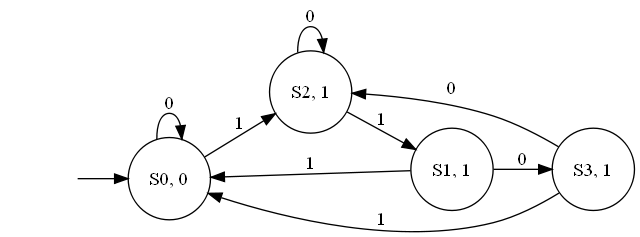
\includegraphics[height=2.0in]{3.png}
	\caption{State diagram for Question 3}
\end{figure}

\section{}

For the Moore machine in question 3, find the output for the given input
strings. I am assuming the start state is S0.

\begin{table}[h!]
	\centering
	\begin{tabular}{ r || r | r }
	Input & Output \\
	\hline      
	$0101$        & $00111$ \\
	$111111$      & $0110110$ \\
	$11101110111$ & $011001100110$ \\
	$1010111$     & $01111011$ \\
	\end{tabular}
	\caption{Output for problem 4.}
	\label{table_3}
\end{table}

\end{document}
